\documentclass[12pt,a4paper]{article}
\usepackage[utf8]{inputenc}
\usepackage[T1]{fontenc}
\usepackage[english, ngerman]{babel}
\usepackage{graphicx}
\usepackage{fancyhdr}
\usepackage{geometry}
\usepackage{setspace}
\usepackage{titlesec}
\usepackage{enumitem}
\usepackage{lmodern}
\usepackage{hyperref}
\usepackage{multicol}

\geometry{left=2.5cm, right=2.5cm, top=2.5cm, bottom=2.5cm}
\pagestyle{fancy}
\fancyhf{}
\rhead{Kagami Kagamiya}
\lhead{Charakterprofil}
\cfoot{\thepage}

\titleformat{\section}{\normalfont\Large\bfseries}{\thesection}{1em}{}
\titleformat{\subsection}{\normalfont\large\bfseries}{\thesubsection}{1em}{}

\hypersetup{
    colorlinks=true,
    linkcolor=black,
    urlcolor=blue
}

\begin{document}

% Deckblatt
\begin{titlepage}
    \centering
    \vspace*{2cm}
    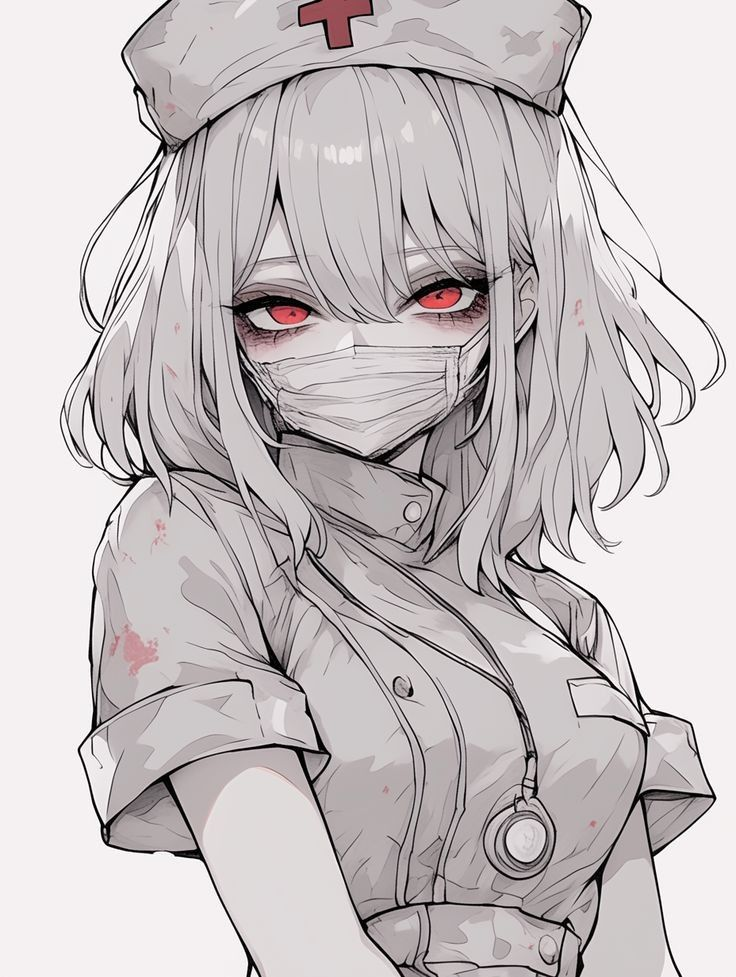
\includegraphics[width=0.5\textwidth]{kagami.jpg}\\[1.5cm]
    {\Huge\bfseries Kagami Kagamiya}\\[0.5cm]
    {\Large Charakterbuch}\\[2cm]
    \vfill
    \textsc{Rasse:} Waldelfe (Albino) \\
    \textsc{Alter:} 25 Jahre \\
    \textsc{Beruf:} Apothekerin und freiwillige Ärztin \\
    \textsc{Setting:} Mittelalterlich, Fantasywelt \\
    \vfill
    \today
\end{titlepage}

\newpage
\tableofcontents
\newpage

% Steckbrief
\section*{Charaktersteckbrief}
\begin{description}[style=nextline]
  \item[Name:] Kagami Kagamiya
  \item[Rasse:] Waldelfe (Albino)
  \item[Alter:] 25 Jahre
  \item[Herkunft:] Dorf nahe [Stadt], im Land [Land] auf dem Kontinent [Kontinent]
  \item[Beruf:] Apothekerin und freiwillige Ärztin
  \item[Aussehen:] Blasses weißes Haar, rote Augen, meist mit Maske. Trägt schlichte, praktische Kleidung. Die Haut ist bleich und empfindlich.
  \item[Charakter:] Ruhig, gelassen – aber leidenschaftlich und neugierig, wenn es um Medizin geht.
  \item[Glaube:] Atheistin
  \item[Ziele:] Wissen über Medizin erweitern, Menschen helfen, Krankheiten verstehen und heilen
\end{description}

\newpage

% Hintergrundgeschichte
\section{Hintergrundgeschichte}

Kagami Kagamiya wurde im kleinen Dorf [Dorf] geboren, wo ihre Familie seit Generationen lebt. Obwohl Elfen in vielen Teilen der Welt kritisch beäugt werden, hat ihre Familie sich durch Bescheidenheit und Hilfsbereitschaft den Respekt der Dorfgemeinschaft erarbeitet. 

Ihr Vater ist ein bodenständiger Schmied, der für das Dorf Waffen, Werkzeuge und Geräte schmiedet. Ihre Mutter bewirtschaftet den großen Garten hinter dem Haus, kennt viele Kräuter – aber nie so im medizinischen Sinne. Kagami entwickelte schon früh eine Faszination für Krankheiten, Wunden und die Geheimnisse des Körpers.

Als sie zwölf war, kam eine reisende Kräuterfrau durch das Dorf. Diese blieb nur einige Tage, aber Kagami sog jedes Wort auf und erhielt ein kleines Bündel handgeschriebener Notizen als Abschiedsgeschenk. Diese Notizen wurden ihr erster "Lehrmeister".

Seitdem erforscht sie selbstständig: durch Lesen, Ausprobieren – und auch Selbstversuche. Manch einer im Dorf tuschelt über ihre Neugier, doch alle respektieren sie spätestens dann, wenn sie mit einem heilenden Sud Fieber brechen oder eine Blutung stillen kann.

\newpage

\section{Welt und Umfeld}

Die politische Ordnung ihres Landes sieht die Elfen über dem Adel, zumindest offiziell. In der Stadt [Stadt] und den angrenzenden Grenzgebieten ist dieses System jedoch umgekehrt oder wird von den Menschen bewusst ignoriert.

Im Dorf herrscht eine gewisse Neutralität. Solange man niemandem schadet, ist Herkunft oder Stand zweitrangig. Kagami genießt daher Narrenfreiheit – nicht, weil sie über allem steht, sondern weil sie gebraucht wird. Und sie missbraucht dieses Vertrauen nicht.

Sie lebt in einem kleinen Haus mit Kräutergarten, weit genug vom Zentrum entfernt, um in Ruhe forschen zu können, aber nahe genug, um im Notfall gerufen zu werden.

\newpage

\section{Motivation und Ziele}

Kagami ist keine Heldin im klassischen Sinne. Sie ist keine Kriegerin, keine Zauberin – und doch fühlt sie sich einem höheren Ziel verpflichtet: dem Leben selbst. Sie glaubt nicht an Götter, sondern an Ursache und Wirkung, an Wissen und Fortschritt.

Ihr größter Traum ist es, ein vollständiges Buch über Krankheiten, Heilmethoden und ihre Erfahrungen zu schreiben – ein medizinisches Werk, das Leben retten kann. Dafür möchte sie in ferne Länder reisen, neue Kulturen und ihre Heilmethoden kennenlernen, seltene Krankheiten erforschen und altes Wissen sammeln.

Sie schließt sich Abenteurern nicht wegen des Goldes an, sondern wegen der Möglichkeiten: Wunden zu behandeln, Wissen zu sammeln, Leben zu retten – und Geschichten zu erleben.

\newpage

\section{Tagebucheinträge}

\subsection*{Eintrag \#17 – Die wandernde Heilerin}

\begin{quote}
Heute kam eine alte Frau ins Dorf – sie trug mehr in ihren Augen als in ihrem Wagen. Ihre Hände zitterten, aber sie kannte Kräuter, die ich nie gesehen habe. Sie nannte sie "Zahnkraut" und "Kriecherblüte". Ich durfte ihre Aufzeichnungen lesen. Sie ließ sie mir da. Ich… ich weiß nicht, ob sie wusste, dass sie stirbt. Aber ich werde sie bewahren. Für sie. Für mich.
\end{quote}

\subsection*{Eintrag \#38 – Selbstversuch \#2}

\begin{quote}
Zubereitung: Tee aus getrockneten Kiefernnadeln, zerriebenem Ingwer und Alkohol.  
Wirkung: Brennt wie Feuer. Aber ich kann wieder klarer denken.  
Nebenwirkung: Übelkeit. Zittern. Werde es verfeinern.
\end{quote}

\newpage

\section{Anhang: Notizen und Rezepturen}

\subsection*{Blutstillender Sud}
\begin{itemize}
  \item 3 Blätter Beerenwurz
  \item 2 Tropfen Harzöl
  \item Prise gemahlene Kohle
  \item In heißem Wasser ziehen lassen – nicht kochen!
\end{itemize}

\subsection*{Fiebertrank}
\begin{itemize}
  \item Schale einer getrockneten Dornsichel
  \item 5 getrocknete Apfelbeeren
  \item Minzsaft
  \item Nach Sonnenuntergang einnehmen
\end{itemize}

\vfill

\begin{center}
    \textit{“Nicht Magie heilt – sondern Wissen.”} \\
    -- Kagami Kagamiya
\end{center}

\end{document}